\section{Zusätzliche Informationen}

Hier können Sie Ihren Anhang definieren.

Achten Sie darauf, dass der Anhang in Ihrer \texttt{thesis.tex}
initial auskommentiert ist.
Der entsprechende Part befindet sich nahe dem Ende der Datei.
Entfernen Sie bei Bedarf die Kommentierung um den Anhang nutzen zu können.


\section{Nutzung}

Der Anhang wird wie die Abschnitte des Hauptteils der Arbeit gestaltet,
also mit \texttt{\textbackslash section} Befehlen.

  \subsection{Unterabschnitte}
  Die Verwendung von Unterabschnitten im Anhang
  mittels \texttt{\textbackslash subsection}
  funktioniert ebenfalls!

\section{Bibliographie}%
\label{app:sec:bib}

Während ihrer Literatur-Recherche werden Sie vermutlich hauptsächlich auf vier Arten
an Quellen stoßen, die Sie in der \verb|.bib|-Datei unterbringen:
Konferenz-Artikel, Sammlungen an Kapiteln von mehreren Autoren, Journal-Artikel und Monographien.
Manche Bibtex-Einträge (etwa von Google Scholar) enthalten nicht alle Informationen
bzw. nicht im selben Format.

\textbf{Wichtig: Eine saubere Bibliographie besteht aus vollständigen und einheitlichen Einträgen!}

Im Folgenden wird beschrieben, was Sie hier für eine möglichst saubere Literaturliste beachten sollten.

\subsection{Konferenzartikel}

In der Informatik wird die meiste Forschung auf Konferenzen vorgestellt.
Hier reichen Autoren ihre Arbeiten ein, andere Forscher begutachten diese
und anhand dessen werden die besten Arbeiten für Konferenzvorträge ausgewählt.
In der Regel gibt es dazu Tagungsbände, die sogenannten \emph{Proceedings},
in denen die vorgestellten Forschungsartikel gesammelt werden.

\begin{figure}
    \centering
    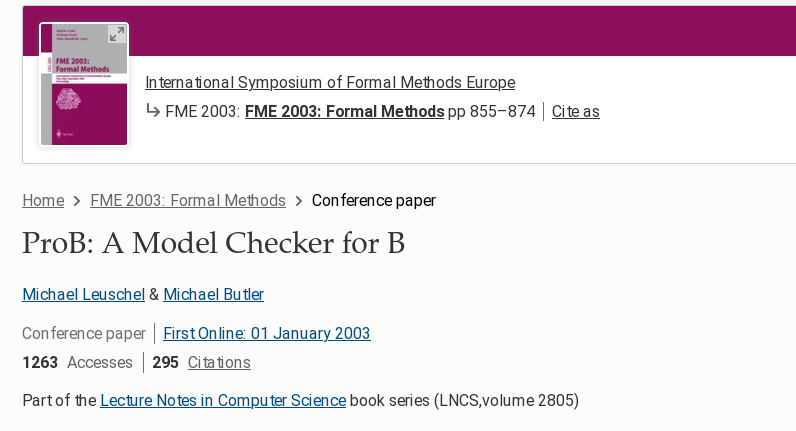
\includegraphics[scale=.5]{fig/prob-springer.png}
    \caption[Screenshot von \url{https://link.springer.com}]{
      Screenshot von \url{https://link.springer.com/chapter/10.1007/978-3-540-45236-2_46}}%
    \label{fig:prob-springer}
\end{figure}

Ein Beispiel ist der Artikel von Leuschel und Butler zu \textsc{ProB}~\cite{leuschel2003prob}.
In \cref{fig:prob-springer} sind die wichtigen Informationen für den Bibtex-Eintrag zu finden,
die Sie auf jeden Fall angeben sollten.
Ein Beispiel für einen passenden Bibtex-Eintrag lautet wie folgt (hier wird der \verb|InProceedings|-Typ verwendet):

\begin{verbatim}
@InProceedings(leuschel2003prob,
  Author	= {Leuschel, Michael and Butler, Michael},
  Title		= {{ProB}: A Model Checker for {B}},
  Year		= 2003,
  Month		= sep,
  Booktitle	= {{FME} 2003: Formal Methods},
  Series	= {LNCS},
  Volume	= 2805,
  Pages		= {855--874},
  Publisher	= {Springer},
  Address	= {Berlin, Heidelberg}
)
\end{verbatim}

\paragraph{Title, Author, Pages.} Diese Einträge sollten selbsterklärend sein.
\paragraph{Booktitle.} Hier gibt es mehrere valide Möglichkeiten.
Auf dem Buch selbst steht \enquote{FME 2003: Formal Methods}.
Akzeptabel wären auch \enquote{Proceedings FME 2003},
\enquote{Proceedings Formal Methods Europe (2003)},
\enquote{International Symposium of Formal Methods Europe. Pisa Italy, September 8-14, 2003, Proceedings}
oder Mischformen.
Wichtig ist, dass erkenntlich ist, zu welcher Konferenz aus welchem Jahr der Tagungsband stammt.
\paragraph{Year.} Leider erscheinen die Proceedings nicht unbedingt im selben Jahr wie die Konferenz selbst.
Daher ist auch das Jahr der Veröffentlichung anzugeben.
\paragraph{Series und Volume}. Proceedings vom Springer-Verlag erscheinen in der Regel in einer Reihe.
Üblich sind die LNCS (Lecture Notes in Computer Science). Darin erhalten sie auch eine Nummer, um sie eindeutig zu identifizieren.
Es gibt aber auch andere Reihen (z.B. LNAI oder CCIS); manchmal werden Tagungsbände auch mehreren Reihen zugeordnet.
Andere Herausgeber haben keine solche Reihe --- dann fallen diese Einträge weg.
\paragraph{Publisher.} Der Herausgeber der Proceedings.
Die meisten Tagungsbände werden vom Springer-Verlag oder der ACM veröffentlicht.
Hier gibt es auch mehrere valide Angaben (z.B. \enquote{Springer} bzw. \enquote{Springer-Verlag} oder \enquote{ACM} bzw. \enquote{Association for Computing Machinery}).
Diese sollten in Ihrer Bibliographie einheitlich sein.



\subsection{Sammelbände}

Es gibt einige Sammlungen an Artikeln, die als thematisches Buch veröffentlicht werden,
allerdings nicht aus einer Konferenz entstehen.
Ein Beispiel ist die Festschrift zu Egon Börgers 75.\ Geburtstag.
Darin findet man unter anderem den folgenden Artikel:

\begin{verbatim}
@InCollection(Leuschel2021,
  Author    = {Leuschel, Michael},
  Title     = {Spot the Difference: A Detailed Comparison Between {B}
                and Event-{B}},
  Booktitle = {Logic, Computation and Rigorous Methods},
  Publisher = {Springer},
  Year      = 2021,
  Volume    = 12750,
  Series    = {Lecture Notes in Computer Science},
  Pages     = {147--172}
)
\end{verbatim}

Insgesamt ist dies sehr ähnlich zum Konferenzartikel; deshalb wird her nicht näher auf die einzelnen Schlüssel eingegangen.
Auch dieses Buch wurde in der LNCS-Reihe veröffentlicht.

\subsection{Journal-Artikel}

Artikel in Journals werden in der Regel als hochwertiger als Konferenz-Artikel angesehen
und sind daher als Quelle zu bevorzugen.
Hier ist die Zeit für die Gutachten in der Regel länger und es wird genauer hingesehen.
Häufig entstehen Journal-Artikel aus Konferenzartikeln und sind ausführlichere Versionen.
Manchmal wird aber auch ohne eine Konferenz-Version direkt in einem Journal eingereicht.

Für die Bibliographie werden viele ähnliche Einträge wie beim Konferenzartikel verwendet,
allerdings ist der Typ hier \verb|Article|.

\begin{verbatim}
@Article(leuschel2008prob,
  Author	= {Leuschel, Michael and Butler, Michael},
  Title		= {{ProB}: An Automated Analysis Toolset for the {B} Method},
  Year		= 2008,
  Month		= mar,
  Journal	= {International Journal on Software Tools for
             Technology Transfer},
  Volume	= 10,
  Pages		= {185--203},
  Number	= 2
)
\end{verbatim}

\paragraph{Title, Author, Pages, Year.} Diese Einträge sollten wieder selbsterklärend sein.
\paragraph{Journal.} Die Artikel werden in einem Journal veröffentlicht, das einen Namen hat.
Hier gibt es in der Regel auch etablierte Abkürzungen (wie etwa \enquote{STTT} für
\enquote{International Journal on Software Tools for Technology Transfer}).
Das Format sollte hier auch einheitlich sein.
\paragraph{Volume und Number.} Journal-Artikel werden meist gesammelt periodisch veröffentlicht.
In der Regel wird die Volume-Zahl pro Jahr erhöht;
innerhalb einer Volume gibt es dann häufig mehrere Veröffentlichungen, die mit der \enquote{issue number} hochgezählt werden.
Wird das Journal also vierteljährlich veröffentlicht, geht der Number-Eintrag bis 4 hoch.
Manchmal gibt es auch \enquote{special issues} zu einem bestimmten Thema oder als Sammlung an Artikeln,
die aus einer bestimmten Konferenz hervorgingen.

\subsection{Monographien}

Einige Bücher werden von vollständig von wenigen Autoren geschrieben.
Hier werden insgesamt recht wenig Informationen benötigt,
wie etwa in dem Beispiel hier:

\begin{verbatim}
@Book(abrial1996b,
  Author	= {Abrial, Jean-Raymond},
  Title		= {The {B}-Book: Assigning Programs to Meanings},
  Year		= 1996,
  Publisher	= {Cambridge University Press},
  Address	= {New York, NY, USA}
)
\end{verbatim}

Leicht andere Arten der Monographien sind Abschlussarbeiten.
Hier haben Master- und Doktorarbeiten eigene Typen mit selbsterklärenden Schlüsseln.
Falls Sie eine Bachelorarbeit zitieren möchten, können Sie auch den Typen \verb|MastersThesis| verwenden.

\begin{verbatim}
@MastersThesis(eulynx_ma,
  Author    = {Abdul Rasheeq},
  Title     = {An Approach To Improve {SysML} Railway Specification
                Using {UML-B} And Event-{B}},
  School    = {Frankfurt University of Applied Sciences},
  Year      = 2019
)
\end{verbatim}

\begin{verbatim}
@PhDThesis(nummenmaa2013executable,
  Author    = {Nummenmaa, Timo},
  Title     = {Executable formal specifications in game development:
                Design, validation and evolution},
  School    = {University of Tampere},
  Year      = 2013
)
\end{verbatim}
